Flow graphs are an abstraction used to represent elements (\eg digital data, goods, electric current) that travel through a network of nodes (\eg computers, physical locations, circuit parts). Flow graphs are often used in the modelling of logistics problems. An attributed flow graph (AFG) is a single-entry/single-exit graph with a \emph{source node} that has no incoming edges and a \emph{sink node} with no outgoing edges.The flow starts in the source node and is directed to the sink node. All other nodes in the AFG, if they exist, must have at least one incoming and one outgoing edge. In addition, AFGs have attributes in their nodes, representing e.g. typec of goods at a given network node, and weights in nodes and edges, representing e.g. the amount of goods stores at that node and flowing between any two nodes. An example of an AFG is shown in Figure~\ref{fig:AFG}.

\begin{figure}[htp]
\centering
\begin{tabular}{cc}
 %   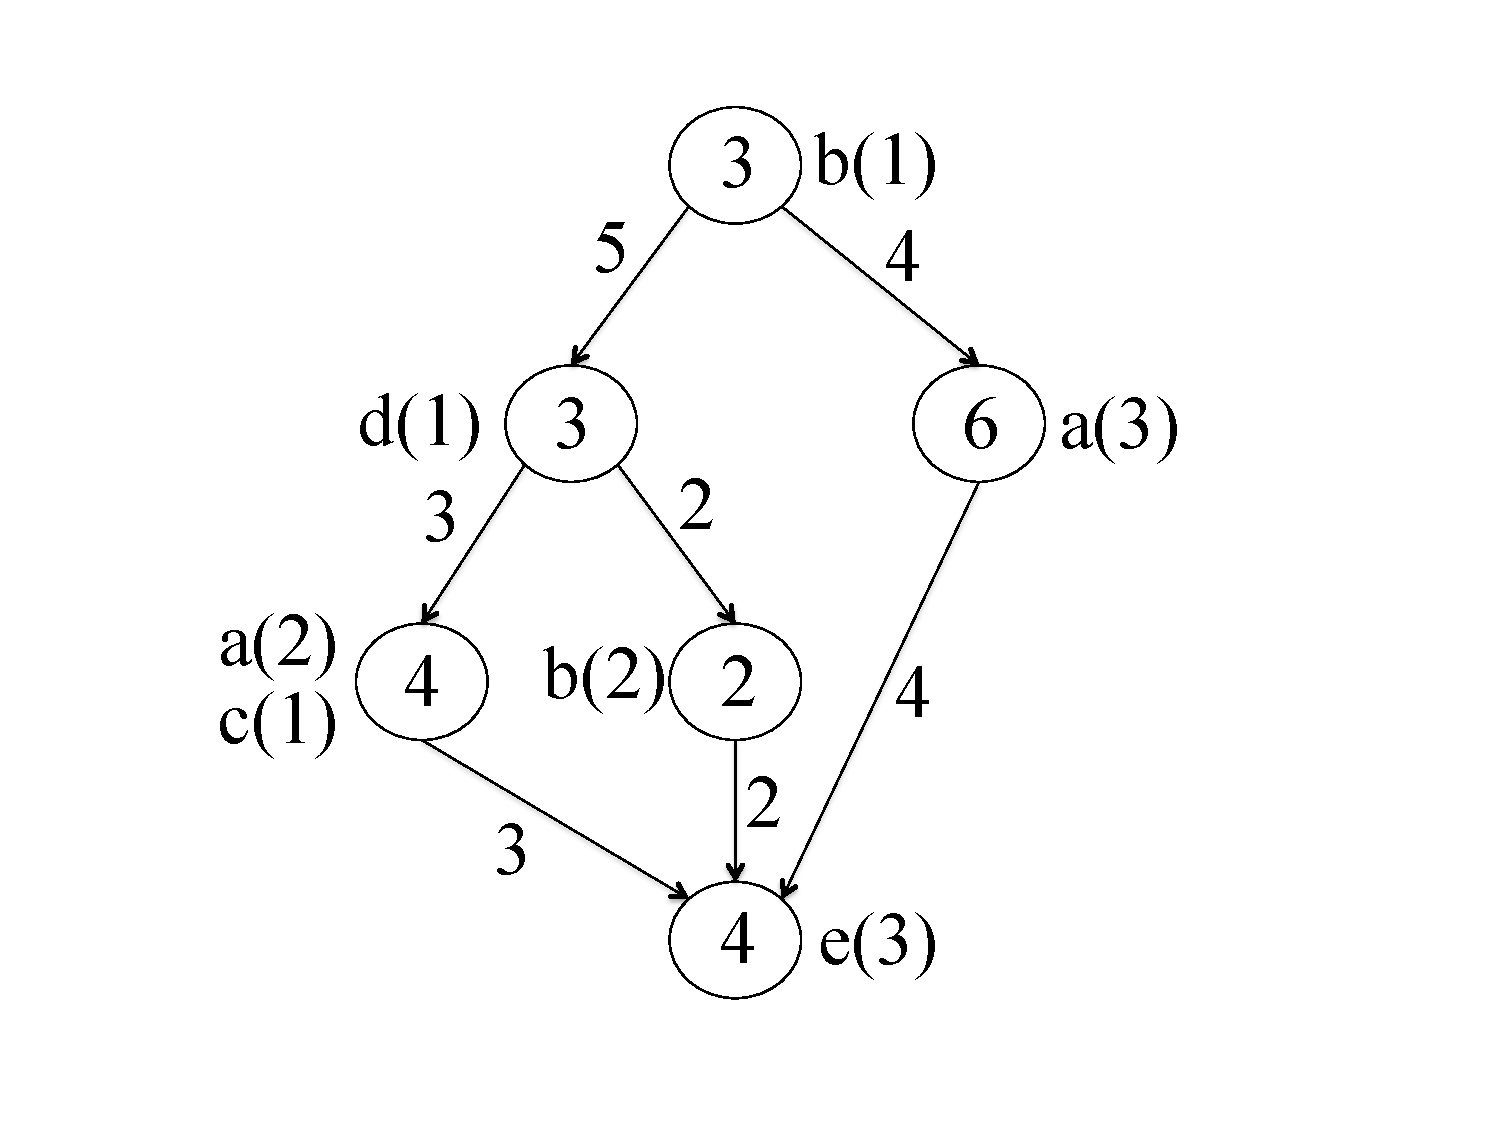
\includegraphics[scale=0.2]{figures/attributed_flow_graph2.eps}
  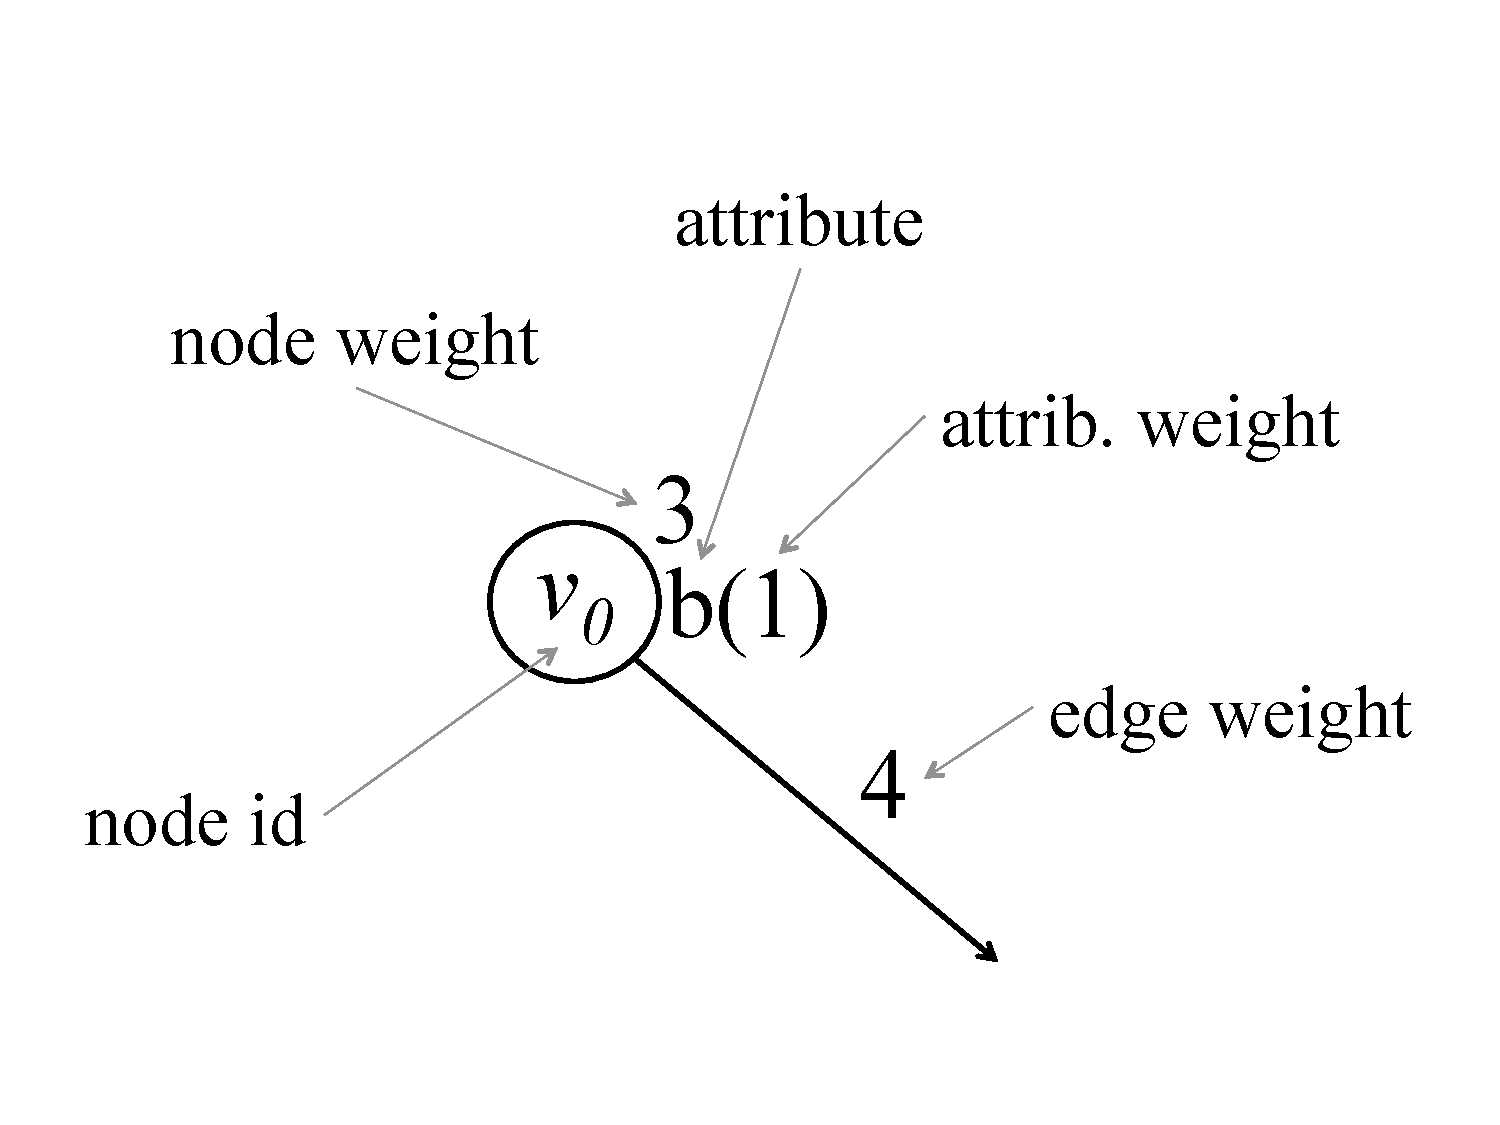
\includegraphics[scale=0.15]{figures/attributed_flow_graph_descpr.pdf} &
  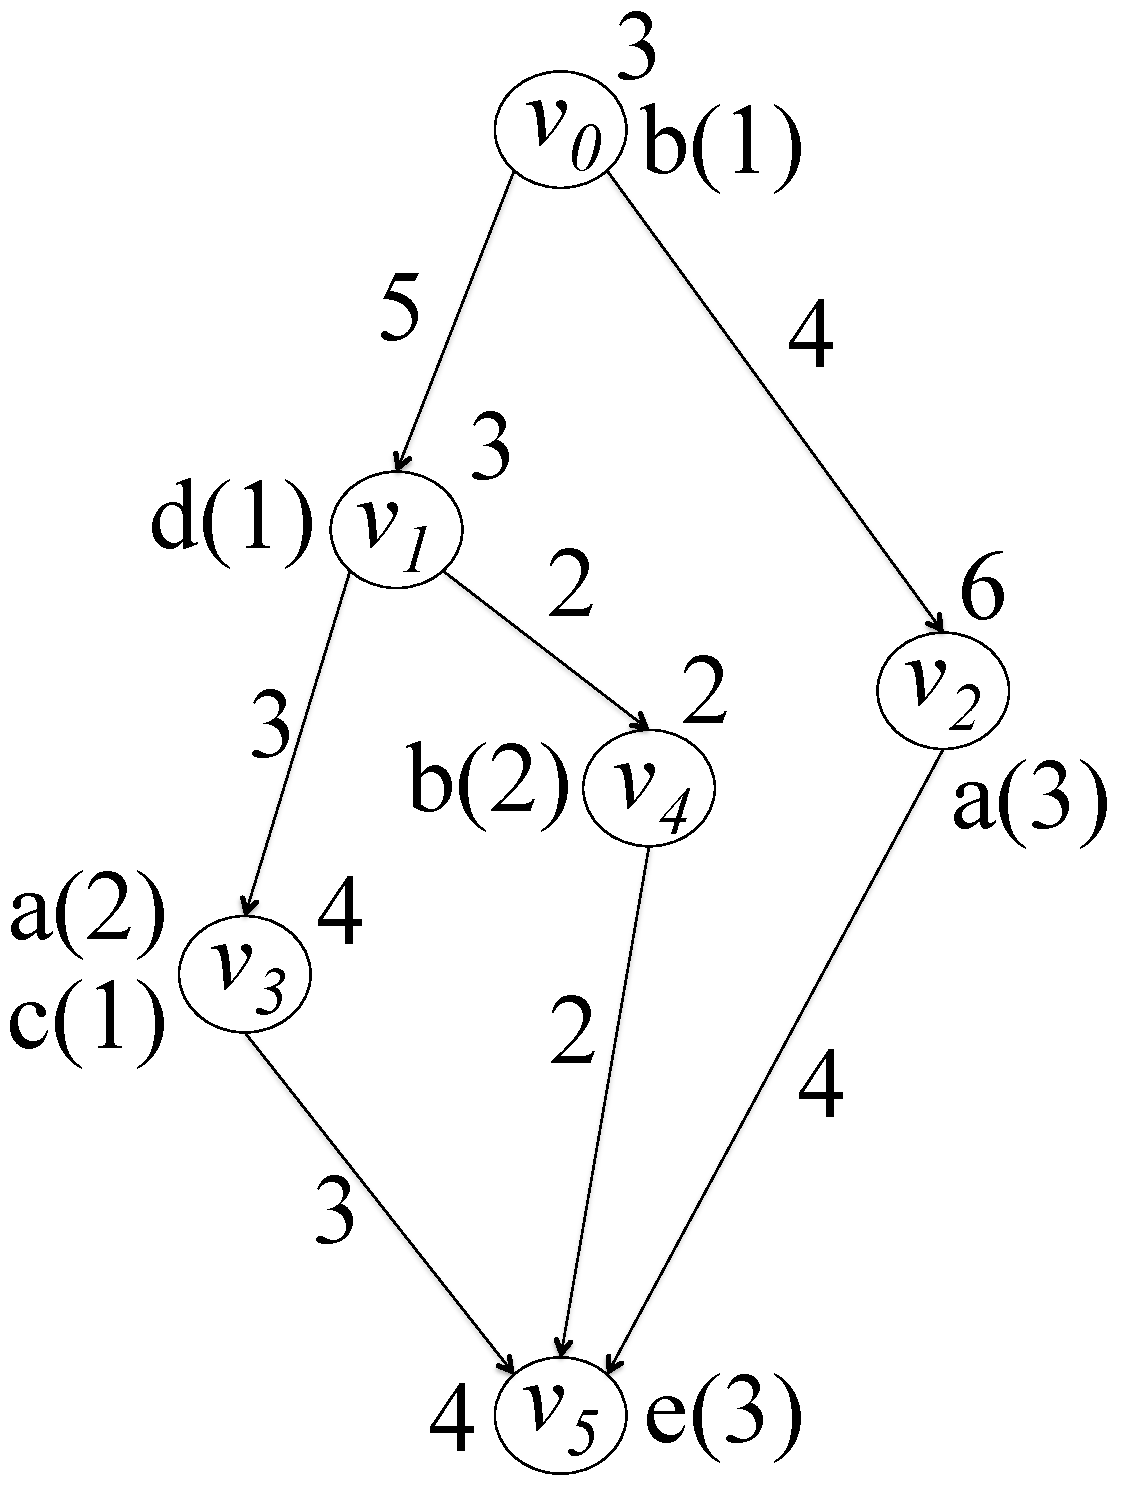
\includegraphics[scale=0.15]{figures/attributed_flow_graph3.pdf}\\
  (a) Elements of an AFG & (b) Example
\end{tabular}
    \caption{Example of attributed flow graph.}
    \label{fig:AFG}  
\end{figure}

Existing graph-mining algorithms are all severely limited in their applicability to AFGs. None of them is able to find general sub-graph patterns in AFGs that take into account multiple node attributes as well as weights in nodes and edges. The only work on mining patterns in AFGs is the FlowGSP algorithm proposed by \emph{Jocksch~\etal}~\cite{FlowGSP}. However, FlowGSP can only find sub-path patterns, while the algorithm described in this work finds all the patterns that FlowGSP does and additional patterns that encompass multiple sub-paths in the dataset.  

This paper presents AFGMiner, the first algorithm, to the best of our knowledge, to address the problem of mining AFGs for general sub-graph patterns. AFGMiner takes as input a set of AFGs and a support measure $MinSup$ that may be formulated by taking into account the attribute weights, node weights and edge weights of the occurrences of patterns. AFGMiner returns all patterns $P$, called \emph{heavyweight patterns}, whose support $MinSup(P)$ is higher than a threshold. This threshold is user-specified as commonly assumed in pattern-mining approaches.
The main contributions of this paper are as follows: 

\begin{enumerate}
\item Definition of the Attributed-Flow-Graph Mining problem to find Heavyweight Patterns.

\item Development of different versions of AFGMiner, an algorithm that mines for heavyweight patterns in attributed flow graphs, including a parallel version with a work-distribution heuristic to maintain workload balance between multiple threads.

\item Development of HEPMiner, a tool that automates the analysis of hardware-instrumented profiles, as an application of AFGMiner. Patterns discovered by HEPMiner indicate potential, non-obvious, opportunities for compiler and architecture-design improvements.

\item Complexity and performance analysis of AFGMiner, comparison against the FlowGSP algorithm and qualitative analysis of patterns found by HEPMiner when applied to the DayTrader benchmark running on IBM's WebSphere Application Server~\cite{WAS}.
\end{enumerate} 




